\begin{figure}[t]
  \centering
  %  row
  \makebox[\linewidth][c]{%
    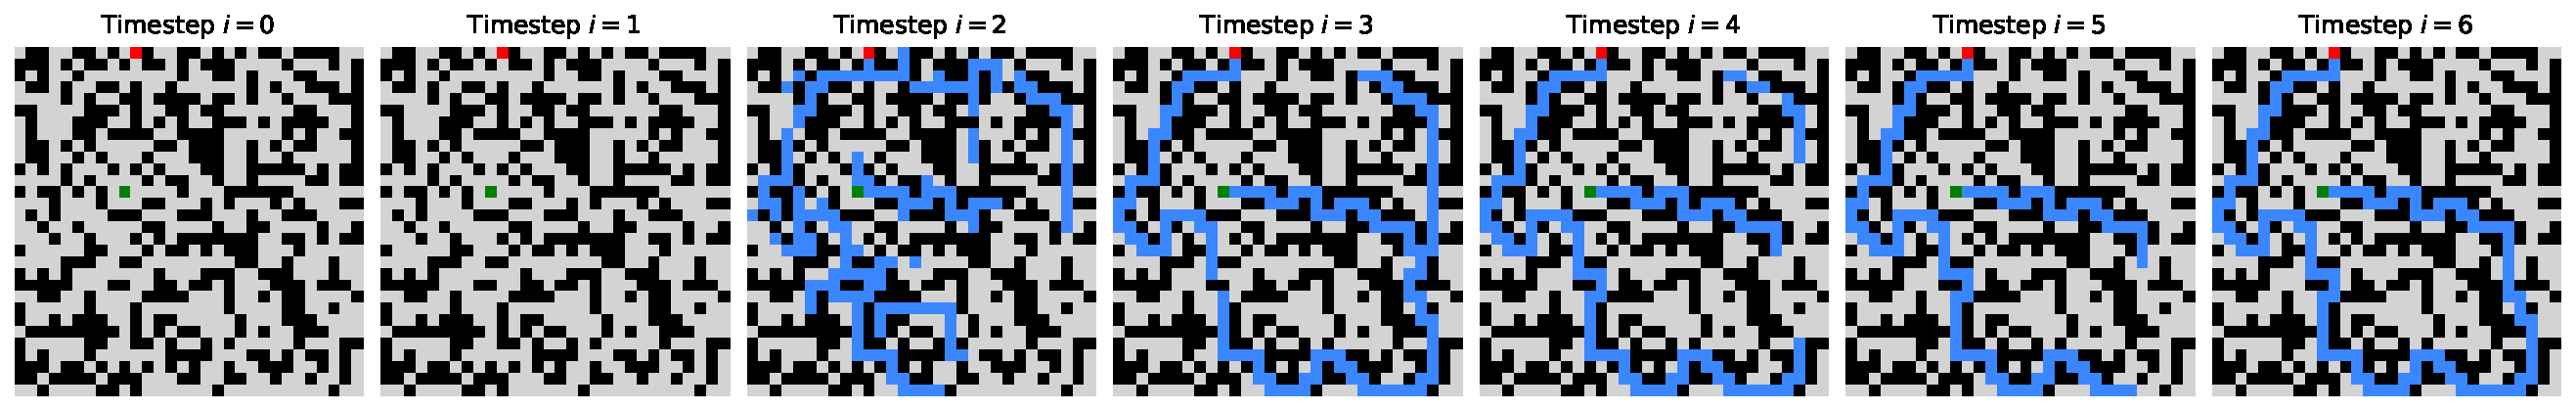
\includegraphics[width=1.1\linewidth]{figures/visualization/maze-100.pdf}%
  }\\
  % row
  \makebox[\linewidth][c]{%
    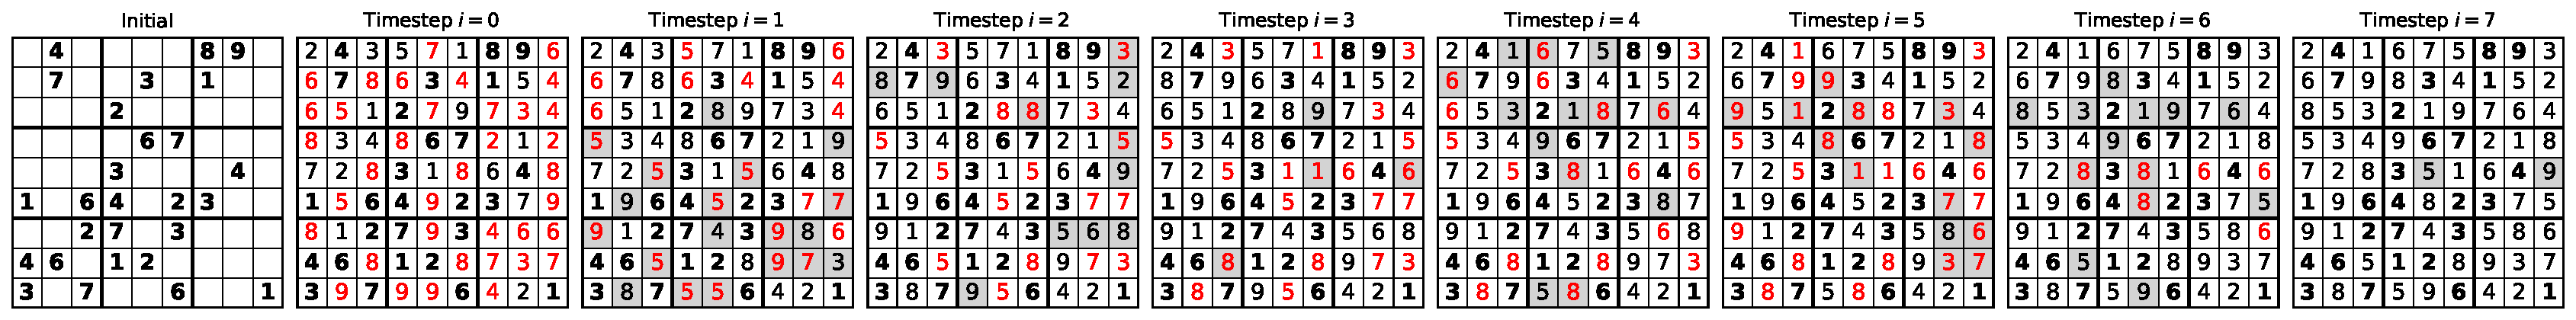
\includegraphics[width=1.1\linewidth]{figures/visualization/sudoku-hard-1.pdf}%
  }\\
    % row
  \makebox[\linewidth][c]{%
    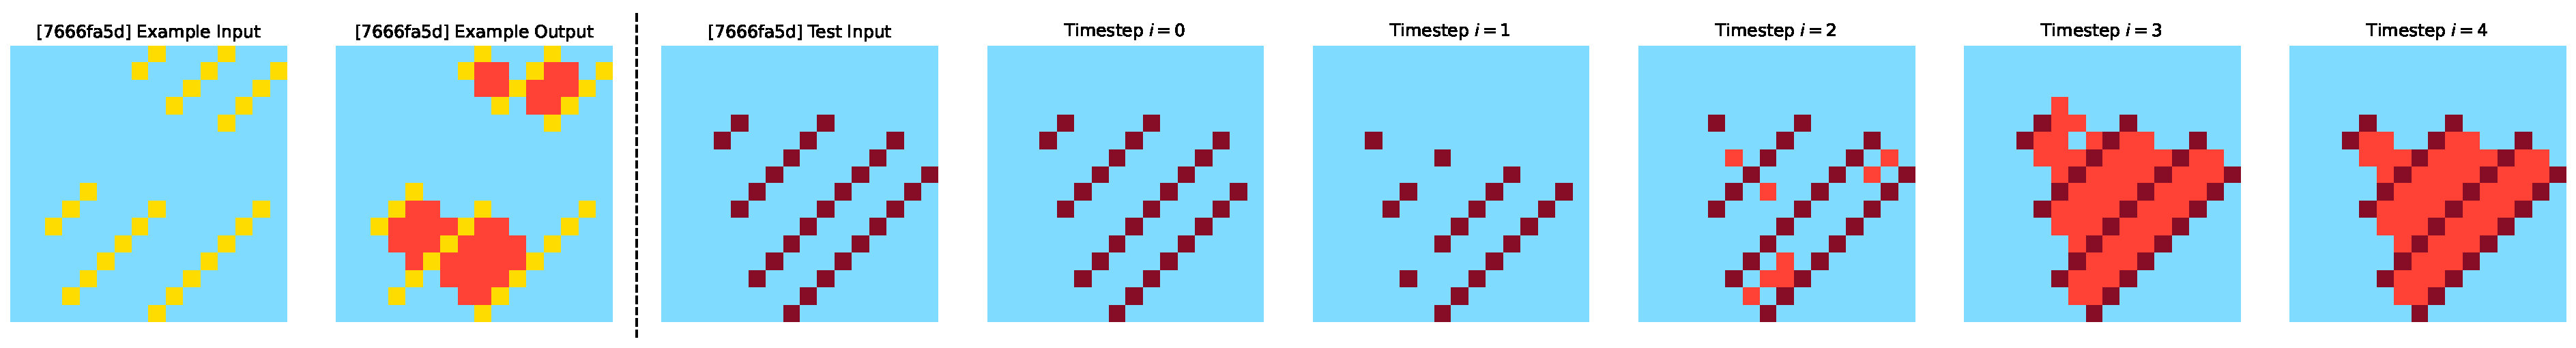
\includegraphics[width=1.1\linewidth]{figures/visualization/7666fa5d.pdf}%
  }\\
      % row
  \makebox[\linewidth][c]{%
    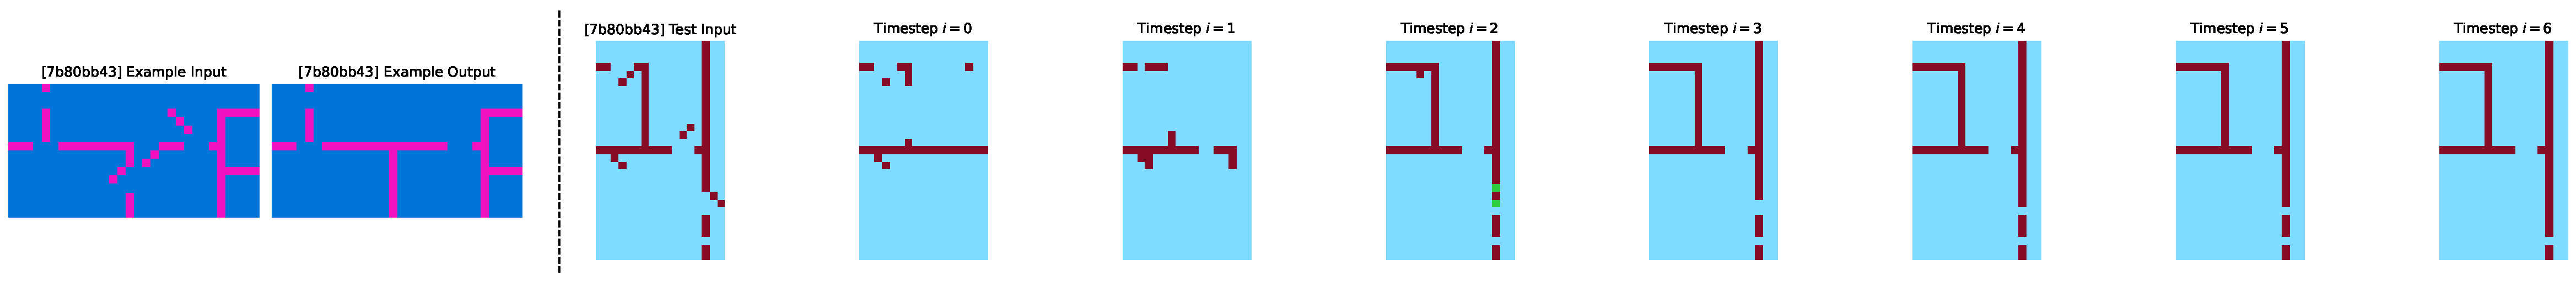
\includegraphics[width=1.1\linewidth]{figures/visualization/7b80bb43.pdf}%
  }
  \caption{\textbf{Visualization of intermediate predictions by HRM on benchmark tasks.} \textbf{Top:} \textit{Maze-Hard}—blue cells indicate the predicted path. \textbf{Middle:} \textit{Sudoku-Extreme}—bold cells represent initial givens; red highlights cells violating Sudoku constraints; grey shading indicates changes from the previous timestep.
  \textbf{Bottom:} ARC-AGI-2 Task—left: provided example input-output pair; right: intermediate steps solving the test input.}
  \label{fig:visualization}
\end{figure}